% Created 2019-11-28 Thu 14:41
% Intended LaTeX compiler: pdflatex
\documentclass[11pt]{article}
\usepackage[utf8]{inputenc}
\usepackage[T1]{fontenc}
\usepackage{graphicx}
\usepackage{grffile}
\usepackage{longtable}
\usepackage{wrapfig}
\usepackage{rotating}
\usepackage[normalem]{ulem}
\usepackage{amsmath}
\usepackage{textcomp}
\usepackage{amssymb}
\usepackage{capt-of}
\usepackage{hyperref}
\author{tigany}
\date{\today}
\title{}
\hypersetup{
 pdfauthor={tigany},
 pdftitle={},
 pdfkeywords={},
 pdfsubject={},
 pdfcreator={Emacs 26.3 (Org mode 9.1.9)}, 
 pdflang={English}}
\begin{document}

\tableofcontents

\section{Narrowed Data for Sasha}
\label{sec:org6e4d328}


\subsubsection{Objective Function}
\label{sec:orgb421cf4}


PARAMETERS
  fdd=0.1958363809 qdds=0.5591275855 qddp=0.5690351902 qddd=0.7745947522 b0=58.0906936439 p0=1.2185323579 b1=-3.2299188646 p1=0.6862915307 b2=593519.1134129359 m2=-11.5000000000 p2=0.0000000000 ndt=2.0000000000 cr1=-6.0000000000 cr2=3.0474400934 cr3=-1.2317472193 r1dd=6.5000000000 rcdd=10.0000000000 rmaxhm=10.1000000000 npar=18 
VARGS
    -vfdd=0.1958363809 -vqdds=0.5591275855 -vqddp=0.5690351902 -vqddd=0.7745947522 -vb0=58.0906936439 -vp0=1.2185323579 -vb1=-3.2299188646 -vp1=0.6862915307 -vb2=593519.1134129359 -vm2=-11.5000000000 -vp2=0.0000000000 -vndt=2.0000000000 -vcr1=-6.0000000000 -vcr2=3.0474400934 -vcr3=-1.2317472193 -vr1dd=6.5000000000 -vrcdd=10.0000000000 -vrmaxhm=10.1000000000 



\begin{center}
\begin{tabular}{lrr}
Quantity & From Model & Target\\
\hline
a\(_{\text{hcp}}\) & 5.58523112 & 5.57678969\\
c/a & 1.58371266 & 1.58731122\\
a\(_{\text{omega}}\) & 8.93475285 & 8.73254342\\
c\(_{\text{omega}}\) & 5.38726911 & 5.32343103\\
a\(_{\text{4h}}\) & 5.57584691 & 5.56325146\\
c\(_{\text{4h}}\) & 18.09810672 & 17.75908031\\
a\(_{\text{6h}}\) & 5.57365569 & 5.54639384\\
c\(_{\text{6h}}\) & 27.18378460 & 26.77136353\\
a\(_{\text{bcc}}\) & 6.20079768 & 6.17948863\\
a\(_{\text{fcc}}\) & 7.87290654 & 7.88677000\\
DE(o,h) & 0.58764167 & -0.63343333\\
DE(4h,h) & 1.58019500 & 3.17160000\\
DE(6h,h) & 2.48264833 & 3.72005000\\
DE(b,h) & 5.35128500 & 7.63520000\\
DE(f,h) & 3.78088500 & 4.51880000\\
c\(_{\text{11}}\) & 171.60928873 & 176.10000000\\
c\(_{\text{33}}\) & 198.90063708 & 190.50000000\\
c\(_{\text{44}}\) & 47.42549704 & 50.80000000\\
c\(_{\text{12}}\) & 94.65941969 & 86.90000000\\
c\(_{\text{13}}\) & 61.22624060 & 68.30000000\\
M\(_{\text{freq}}\)\(_{\text{0}}\) & 2.59341377 & 2.85858719\\
M\(_{\text{freq}}\)\(_{\text{1}}\) & 2.59341378 & 2.85858719\\
M\(_{\text{freq}}\)\(_{\text{2}}\) & 2.59341378 & 2.85858719\\
M\(_{\text{freq}}\)\(_{\text{3}}\) & 2.59341379 & 2.85858719\\
M\(_{\text{freq}}\)\(_{\text{4}}\) & 5.85272461 & 5.66706047\\
M\(_{\text{freq}}\)\(_{\text{5}}\) & 5.85272461 & 5.66706047\\
H\(_{\text{freq}}\)\(_{\text{0}}\) & 3.82320403 & 4.80643423\\
H\(_{\text{freq}}\)\(_{\text{1}}\) & 3.82320403 & 5.58010025\\
H\(_{\text{freq}}\)\(_{\text{2}}\) & 6.40288977 & 5.65316738\\
H\(_{\text{freq}}\)\(_{\text{3}}\) & 6.40288977 & 6.36651842\\
H\(_{\text{freq}}\)\(_{\text{4}}\) & 7.92857431 & 6.40050186\\
H\(_{\text{freq}}\)\(_{\text{5}}\) & 7.92857431 & 7.64082373\\
bandw.  G & 3.69394702 & 5.87085872\\
bandw.  K & 4.65178817 & 4.97424321\\
bandw.  M & 5.19329495 & 7.78109872\\
bandw.  L & 4.21232412 & 6.34433701\\
bandw.  H & 3.54700549 & 9.70902614\\
DOSerr\(_{\text{h}}\) & 0.00000000 & 0.00000000\\
DOSerr\(_{\text{o}}\) & 0.00000000 & 0.00000000\\
E\(_{\text{pris}}\)\(_{\text{f}}\) & 98.95340236 & 220.00000000\\
\end{tabular}
\end{center}



----------     E\(_{\text{prismatic}}\)\(_{\text{fault}}\)     -----------

\begin{center}
\begin{tabular}{lrll}
tbe: & 98.953 & mJ/m\(^{\text{2}}\) & \\
DFT: & 250.000 & mJ/m\(^{\text{2}}\) & [Benoit  2012]\\
DFT: & 233.000 & mJ/m\(^{\text{2}}\) & [Ackland 1999]\\
\end{tabular}
\end{center}


----------     E\(_{\text{Basal}}\)\(_{\text{fault}}\) I2     -----------

\begin{center}
\begin{tabular}{lrll}
tbe: & 211.658 & mJ/m\(^{\text{2}}\) & \\
DFT: & 260.000 & mJ/m\(^{\text{2}}\) & [Benoit  2012]\\
\end{tabular}
\end{center}

\subsubsection{Defect Clusters}
\label{sec:orgb82de00}

----------     E\(_{\text{vacancy}}\)\(_{\text{formation}}\)     ----------

\begin{center}
\begin{tabular}{lll}
tbe: & 2.347  eV & \\
DFT: & 1.950  eV & GGA-PAW:   Angsten  (2013)\\
exp: & 1.270  eV & Hashimoto  (1984)\\
\end{tabular}
\end{center}

\begin{enumerate}
\item Octahedral O interstitial relaxation
\label{sec:orga895f93}

Initial:
\begin{center}
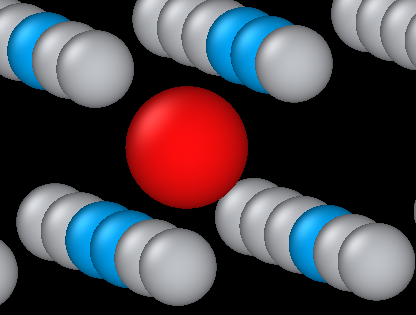
\includegraphics[width=.9\linewidth]{Images/initial_octahedral_ox_ovito.png}
\end{center}

Final:
\begin{center}
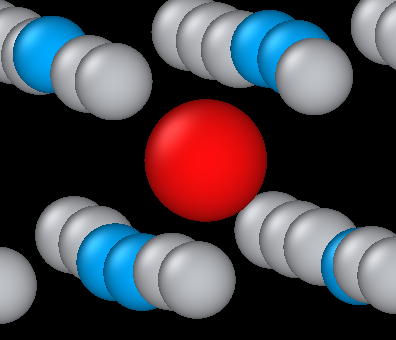
\includegraphics[width=.9\linewidth]{Images/final_octahedral_ox_ovito.png}
\end{center}

\item Tetrahedral O interstitial relaxation
\label{sec:org054b826}

Initial:
\begin{center}
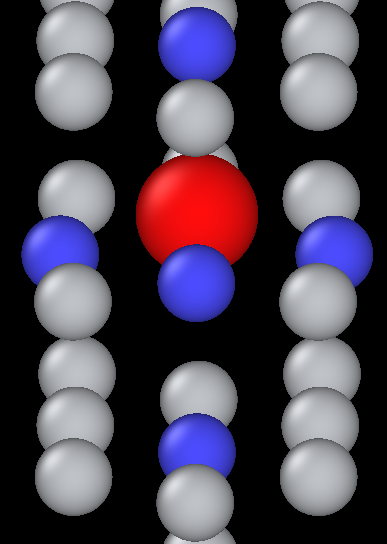
\includegraphics[width=.9\linewidth]{Images/final_model_final_tetra_ox.png}
\end{center}

Final:
\begin{center}
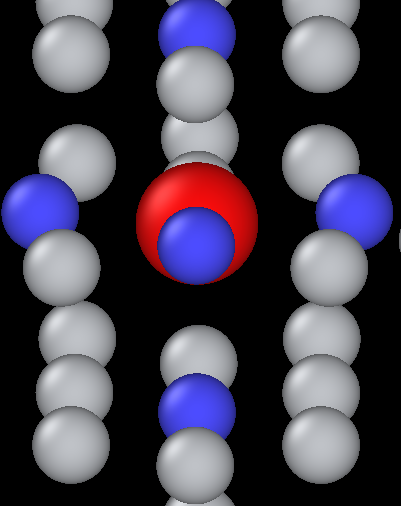
\includegraphics[width=.9\linewidth]{Images/final_model_initial_tetra_ox_ovito.png}
\end{center}


\item Energies for defects
\label{sec:org2edb66d}

Relative differences are 

>> (E\(_{\text{tetrahedral}}\) - E\(_{\text{octahedral}}\)) 
\begin{center}
\begin{tabular}{lll}
tbe: & 1.65 eV & \\
GGA-DFT: & 1.23 eV & Kwasniak (2013)\\
\end{tabular}
\end{center}

>> (E\(_{\text{hexahedral}}\) - E\(_{\text{octahedral}}\))
\begin{center}
\begin{tabular}{ll}
tbe: & 0.90 eV\\
\end{tabular}
\end{center}

> Note: Preference for tetrahedral oxygen to go into hexahedral site as seen by images above

All formation energies below use the chemical potential of Akysonov
(2013) of value \(\mu_{\text{oxygen}} = \frac{5.6}{ 2} eV\).

\item All formation energies
\label{sec:orgf972dca}

\begin{center}
\begin{tabular}{ll}
Quantity & Energy (eV)\\
\hline
Ef\(_{\text{Vf}}\) & 2.347\\
 & \\
Ef\(_{\text{T}}\)\(_{\text{sol}}\) & -  21.783\\
Ef\(_{\text{T}}\)\(_{\text{dil}}\)\(_{\text{imp}}\) & -  28.991\\
Ef\(_{\text{T}}\)\(_{\text{formation}}\) & -  21.783\\
Ef\(_{\text{T}}\)\(_{\text{V}}\)\(_{\text{formation}}\) & -  18.905\\
Ef\(_{\text{T}}\)\(_{\text{vac}}\)\(_{\text{sol}}\)\(_{\text{bind}}\) & -   0.530\\
 & \\
Ef\(_{\text{O}}\)\(_{\text{sol}}\) & -  23.436\\
Ef\(_{\text{O}}\)\(_{\text{dil}}\)\(_{\text{imp}}\) & -  30.645\\
Ef\(_{\text{O}}\)\(_{\text{formation}}\) & -  23.436\\
Ef\(_{\text{O}}\)\(_{\text{V}}\)\(_{\text{formation}}\) & -  18.905\\
Ef\(_{\text{O}}\)\(_{\text{vac}}\)\(_{\text{sol}}\)\(_{\text{bind}}\) & -   2.183\\
 & \\
Ef\(_{\text{OO}}\)\(_{\text{sol}}\) & -  49.606\\
Ef\(_{\text{OO}}\)\(_{\text{dil}}\)\(_{\text{imp}}\) & -  56.814\\
Ef\(_{\text{OO}}\)\(_{\text{formation}}\) & -  46.806\\
Ef\(_{\text{OO}}\)\(_{\text{V}}\)\(_{\text{formation}}\) & -  41.910\\
Ef\(_{\text{OO}}\)\(_{\text{vac}}\)\(_{\text{sol}}\)\(_{\text{bind}}\) & -   2.547\\
 & \\
Ef\(_{\text{OOO}}\)\(_{\text{sol}}\) & -  76.037\\
Ef\(_{\text{OOO}}\)\(_{\text{dil}}\)\(_{\text{imp}}\) & -  83.246\\
Ef\(_{\text{OOO}}\)\(_{\text{formation}}\) & -  70.437\\
Ef\(_{\text{OOO}}\)\(_{\text{V}}\)\(_{\text{formation}}\) & -  66.013\\
Ef\(_{\text{OOO}}\)\(_{\text{vac}}\)\(_{\text{sol}}\)\(_{\text{bind}}\) & -   2.076\\
 & \\
Ef\(_{\text{OOOO}}\)\(_{\text{sol}}\) & - 102.470\\
Ef\(_{\text{OOOO}}\)\(_{\text{dil}}\)\(_{\text{imp}}\) & - 109.679\\
Ef\(_{\text{OOOO}}\)\(_{\text{formation}}\) & -  94.070\\
Ef\(_{\text{OOOO}}\)\(_{\text{V}}\)\(_{\text{formation}}\) & -  88.998\\
Ef\(_{\text{OOOO}}\)\(_{\text{vac}}\)\(_{\text{sol}}\)\(_{\text{bind}}\) & -  2.724\\
 & \\
Ef\(_{\text{OOOOO}}\)\(_{\text{sol}}\) & - 128.781\\
Ef\(_{\text{OOOOO}}\)\(_{\text{dil}}\)\(_{\text{imp}}\) & - 135.989\\
Ef\(_{\text{OOOOO}}\)\(_{\text{formation}}\) & - 117.581\\
Ef\(_{\text{OOOOO}}\)\(_{\text{V}}\)\(_{\text{formation}}\) & - 113.649\\
Ef\(_{\text{OOOOO}}\)\(_{\text{vac}}\)\(_{\text{sol}}\)\(_{\text{bind}}\) & - 1.583\\
 & \\
Ef\(_{\text{OOOOOO}}\)\(_{\text{sol}}\) & - 155.148\\
Ef\(_{\text{OOOOOO}}\)\(_{\text{dil}}\)\(_{\text{imp}}\) & - 162.357\\
Ef\(_{\text{OOOOOO}}\)\(_{\text{formation}}\) & - 141.148\\
Ef\(_{\text{OOOOOO}}\)\(_{\text{V}}\)\(_{\text{formation}}\) & - 137.110\\
Ef\(_{\text{OOOOOO}}\)\(_{\text{vac}}\)\(_{\text{sol}}\)\(_{\text{bind}}\) & - 1.690\\
\end{tabular}
\end{center}
\end{enumerate}

\subsubsection{Gamma surfaces}
\label{sec:org9094bcd}

Energies are accurate to within 2 mJm\(^{\text{-2}}\), comparing the energies of
points in the corners which (the zeros of energy). So surface energies
might be  \(\pm 2\) mJm\(^{\text{-2}}\) off which is reasonable. 

These calculations were done in tight binding with 15 layers for both
basal and prismatic with k-points adjusted accordingly. 
DFT comparisons are usind results of Rodney. 

The Pyramidal surface was obtained using the same 32 atom cell that
Ready used in his paper on the pyramidal gamma surface with DFT
pseudopotentials. 

\newpage
\begin{enumerate}
\item Basal
\label{sec:orgb31c1ab}

TBE:
\begin{center}
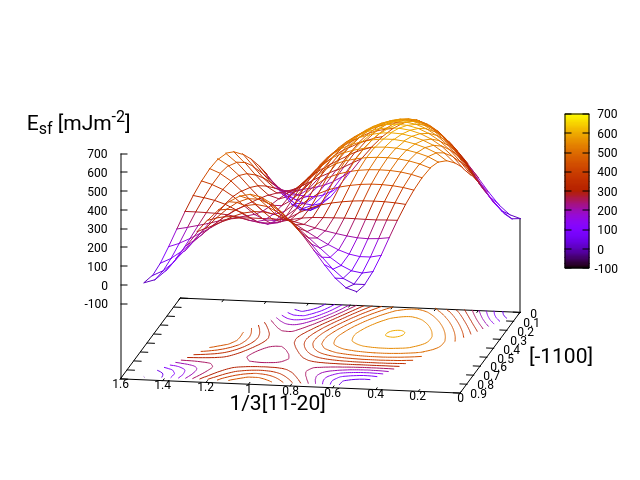
\includegraphics[width=.9\linewidth]{Images/basal_gs_noo_2019-11-08_alat.png}
\end{center}

DFT:
\begin{center}
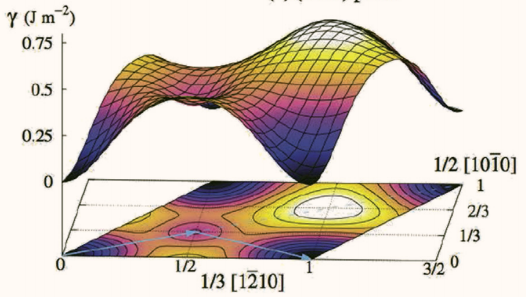
\includegraphics[width=.9\linewidth]{Images/rodney_basal_ti_gamma_surface.png}
\end{center}

\item Prismatic
\label{sec:orgd10b9e2}

TBE:
\begin{center}
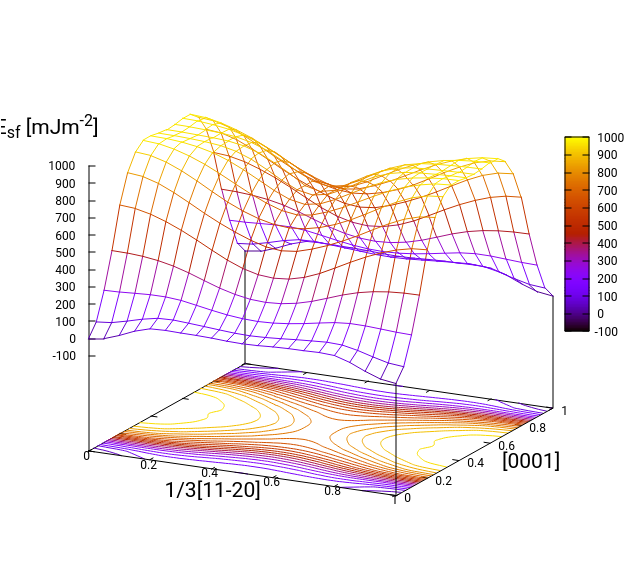
\includegraphics[width=.9\linewidth]{Images/prismatic_gs_noo_2019-11-08_alat.png}
\end{center}

DFT:
\begin{center}
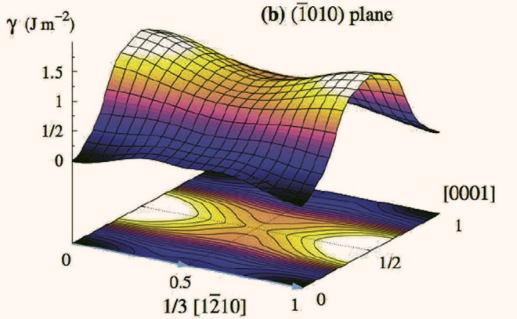
\includegraphics[width=.9\linewidth]{Images/rodney_prismatic_ti_gamma_surface.png}
\end{center}

\item Pyramidal first order
\label{sec:orgecb12bb}

TBE:
\begin{center}
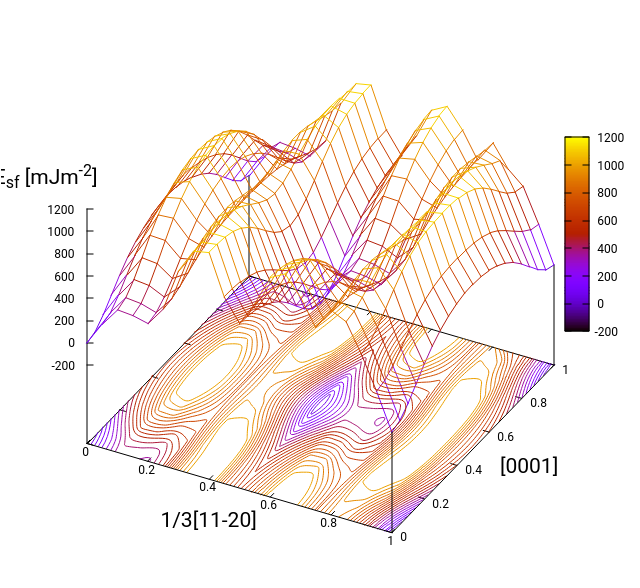
\includegraphics[width=.9\linewidth]{Images/pyramidal_gs_noo_2019-11-08_alat.png}
\end{center}

DFT pseudopot:
\begin{center}
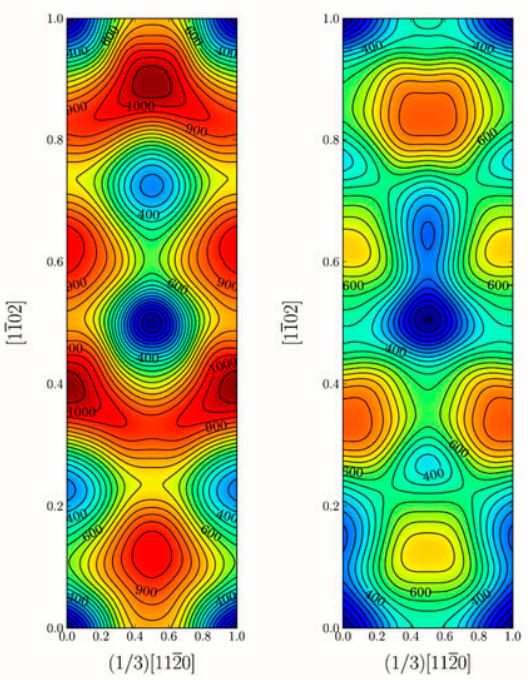
\includegraphics[width=.9\linewidth]{Images/pyramidal_gamma_surface_ready_data_both.png}
\end{center}

\item Data
\label{sec:org92925a0}
\href{file:///home/tigany/Documents/ti/final\_model\_2019-11-12/results\_2019-11-09\_muc/gamma\_surfaces/basal/basal\_gs\_noo\_alat\_energies.dat}{basal\(_{\text{gs}}\)\(_{\text{data}}\)}
\href{file:///home/tigany/Documents/ti/final\_model\_2019-11-12/results\_2019-11-09\_muc/gamma\_surfaces/prismatic/prismatic\_gs\_noo\_alat\_energies.dat}{prismatic\(_{\text{gs}}\)\(_{\text{data}}\)}
\href{file:///home/tigany/Documents/ti/final\_model\_2019-11-12/gamma\_surfaces/pyramidal\_results\_2019-11-13/pyramidal\_gamma\_surface\_2019-11-13.dat}{pyramidal\(_{\text{gs}}\)\(_{\text{data}}\)}
\end{enumerate}
\subsubsection{Dislocation core structures}
\label{sec:org71c179b}
\begin{center}
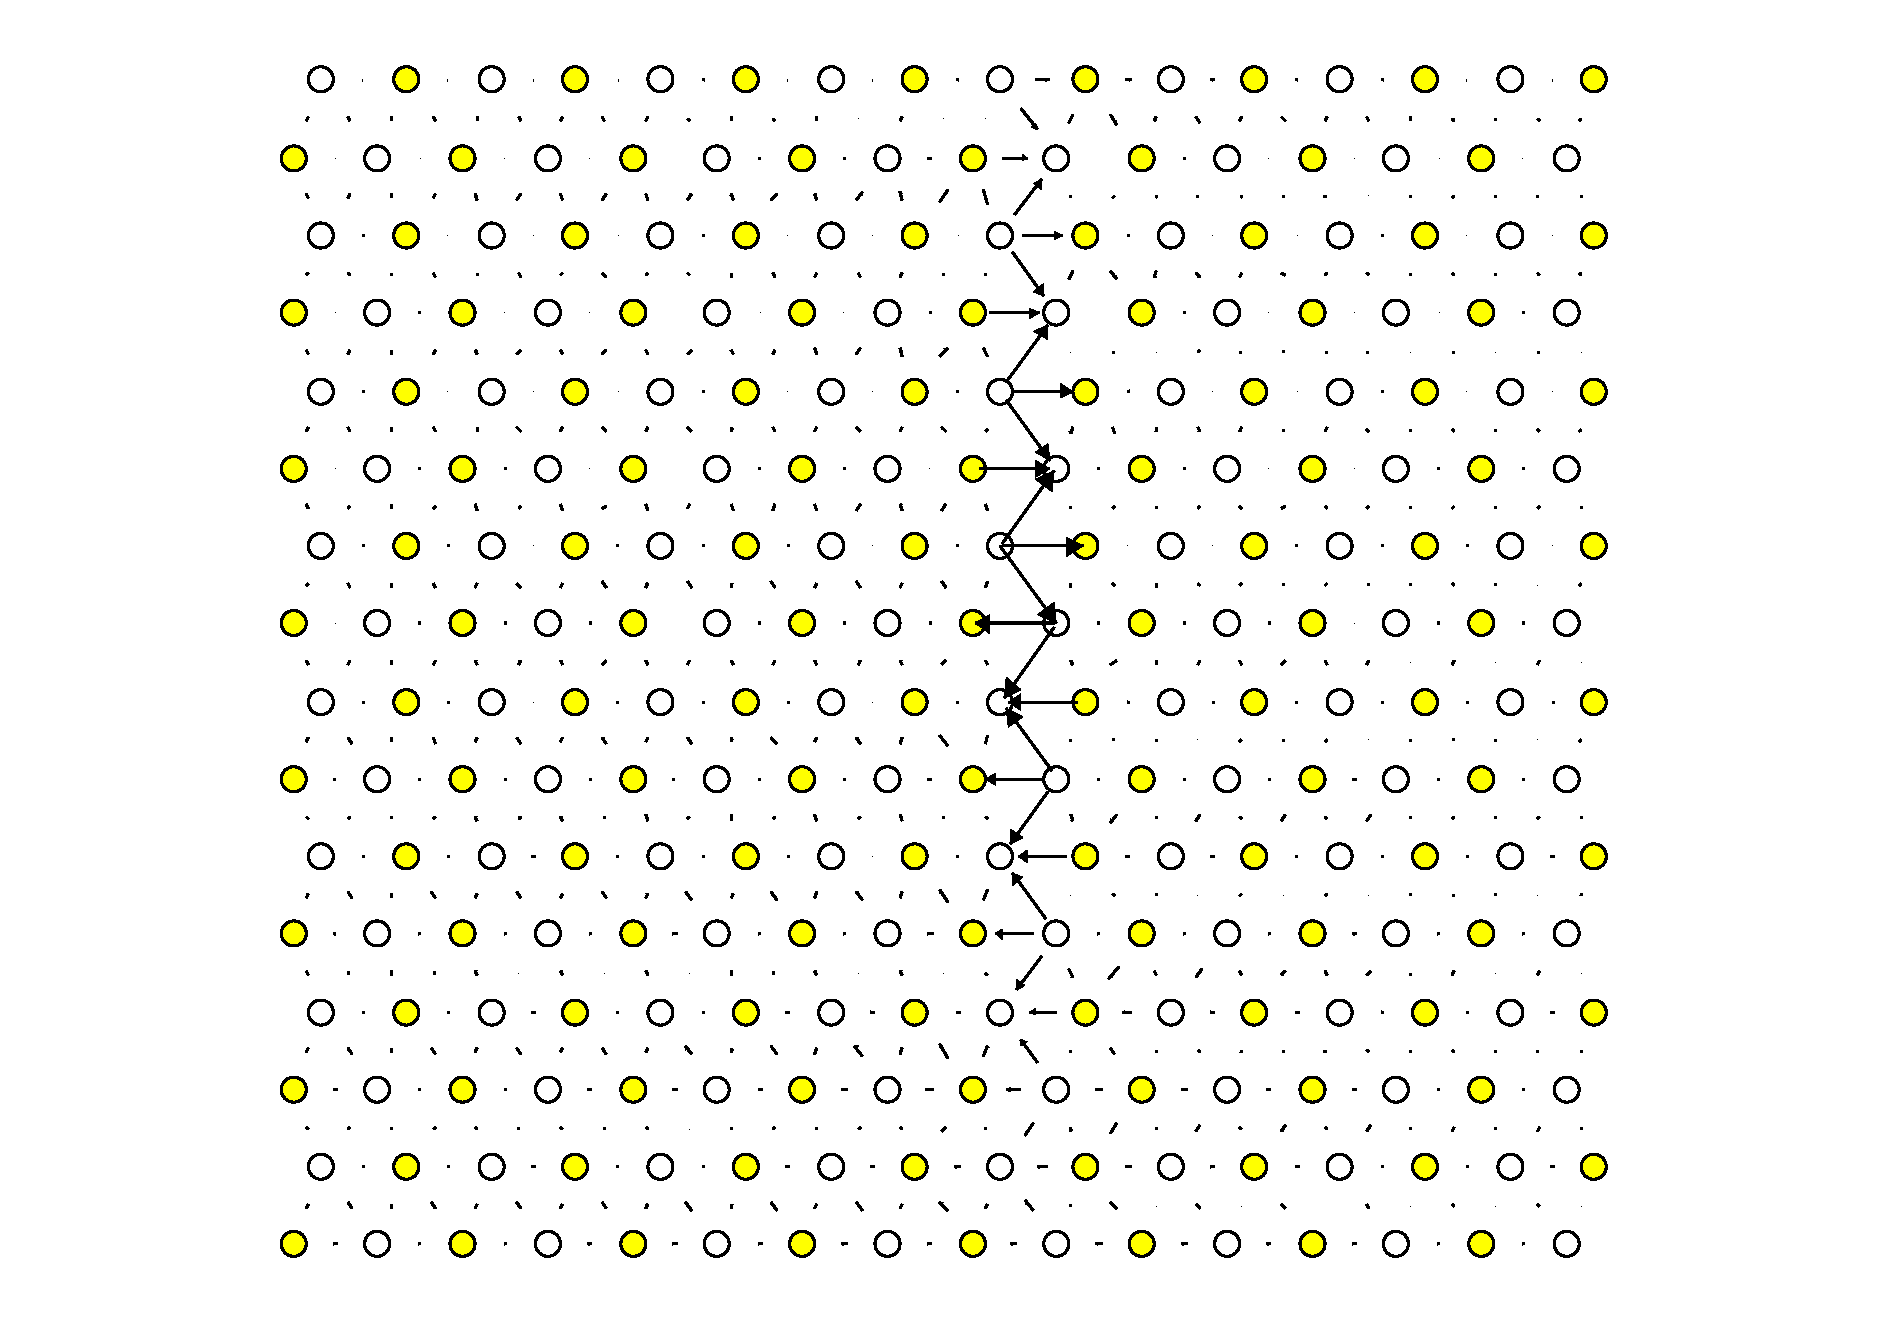
\includegraphics[width=.9\linewidth]{Images/ddplot_IP1_noo_best_model_alat.eps}
\end{center}
\begin{center}
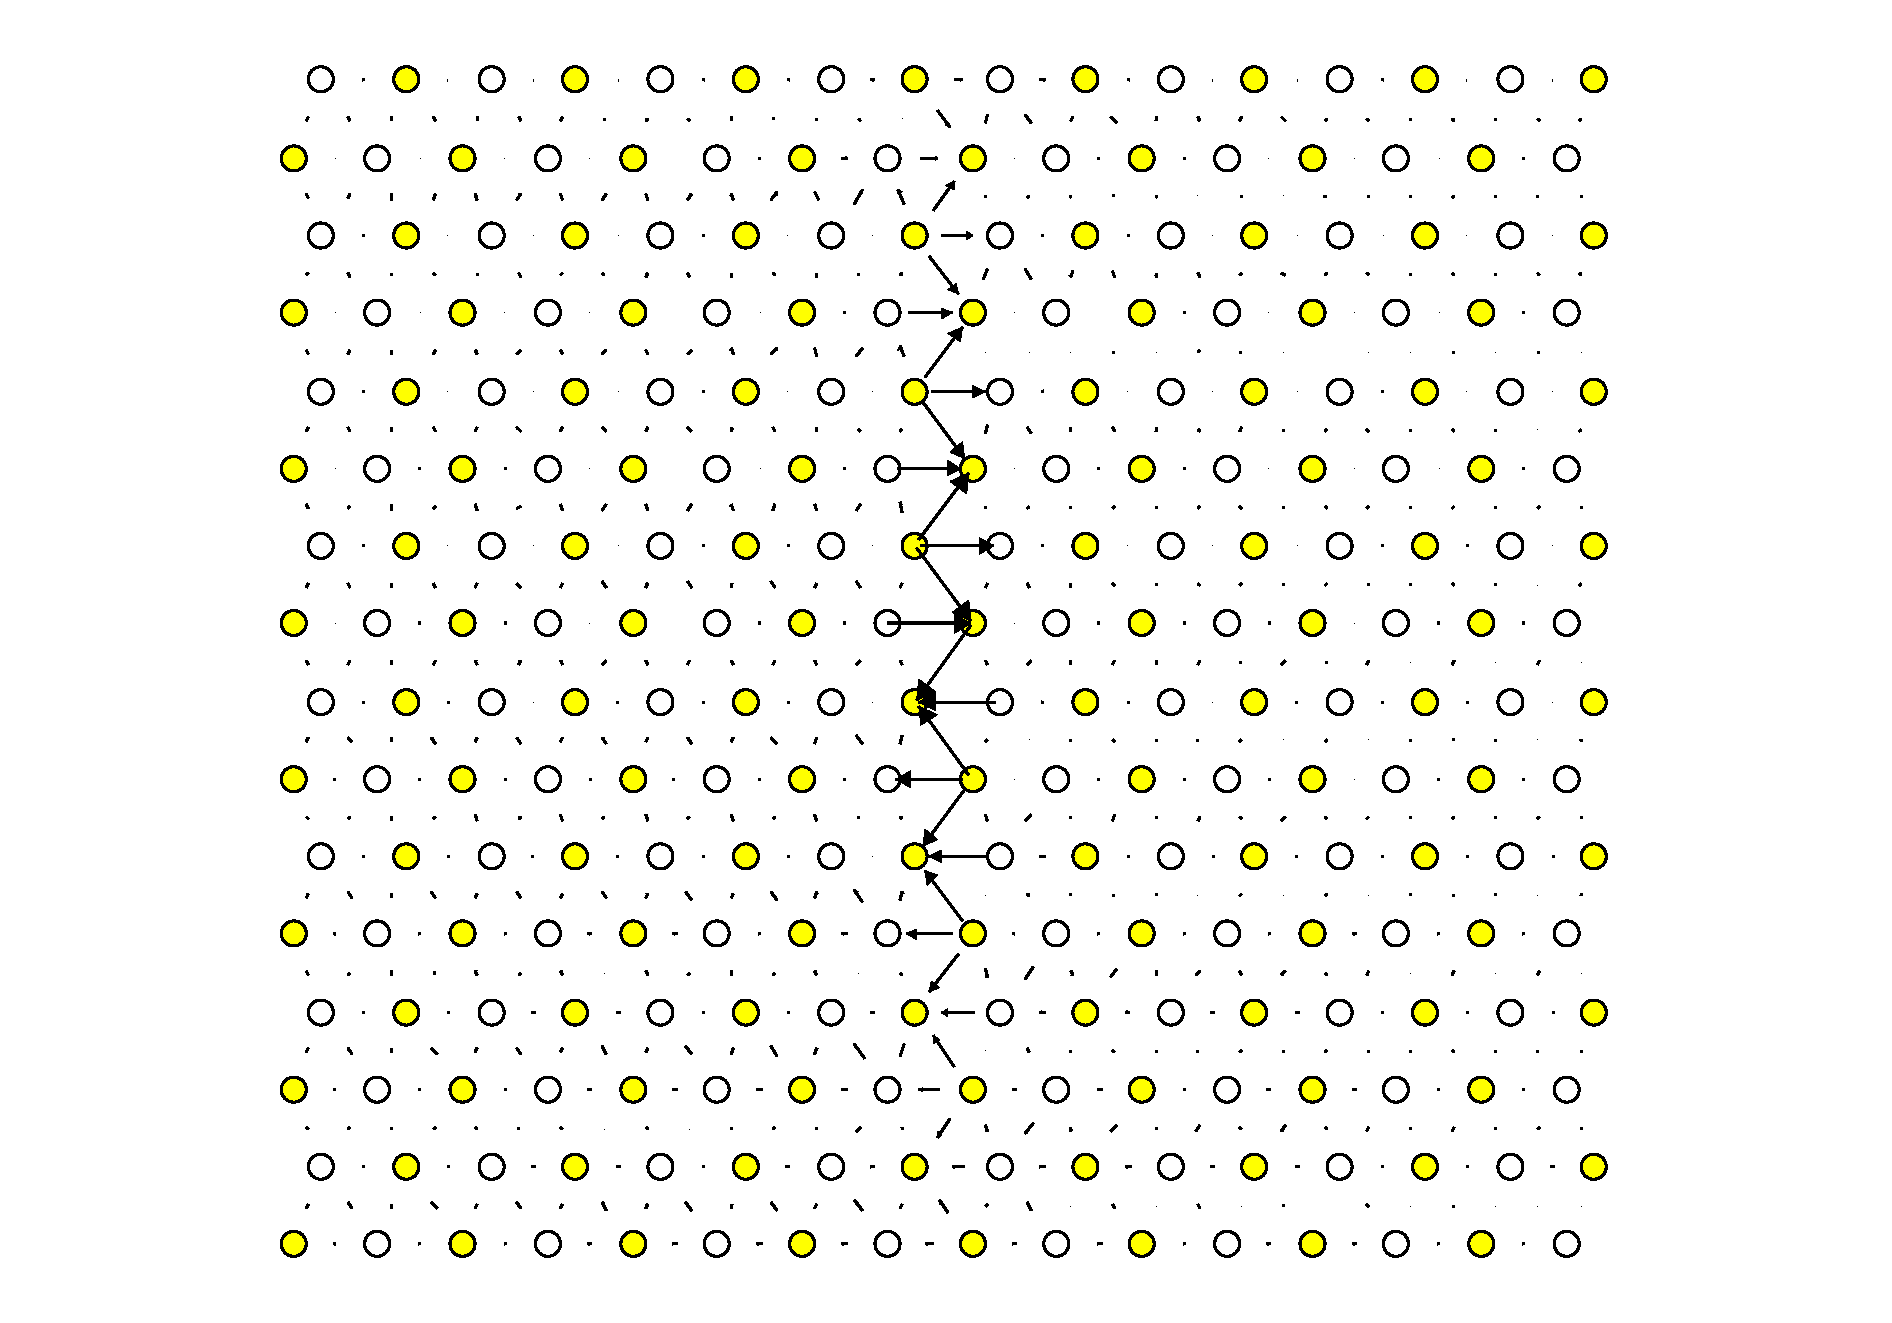
\includegraphics[width=.9\linewidth]{Images/ddplot_IP2_noo_best_model_alat.eps}
\end{center}
\begin{center}
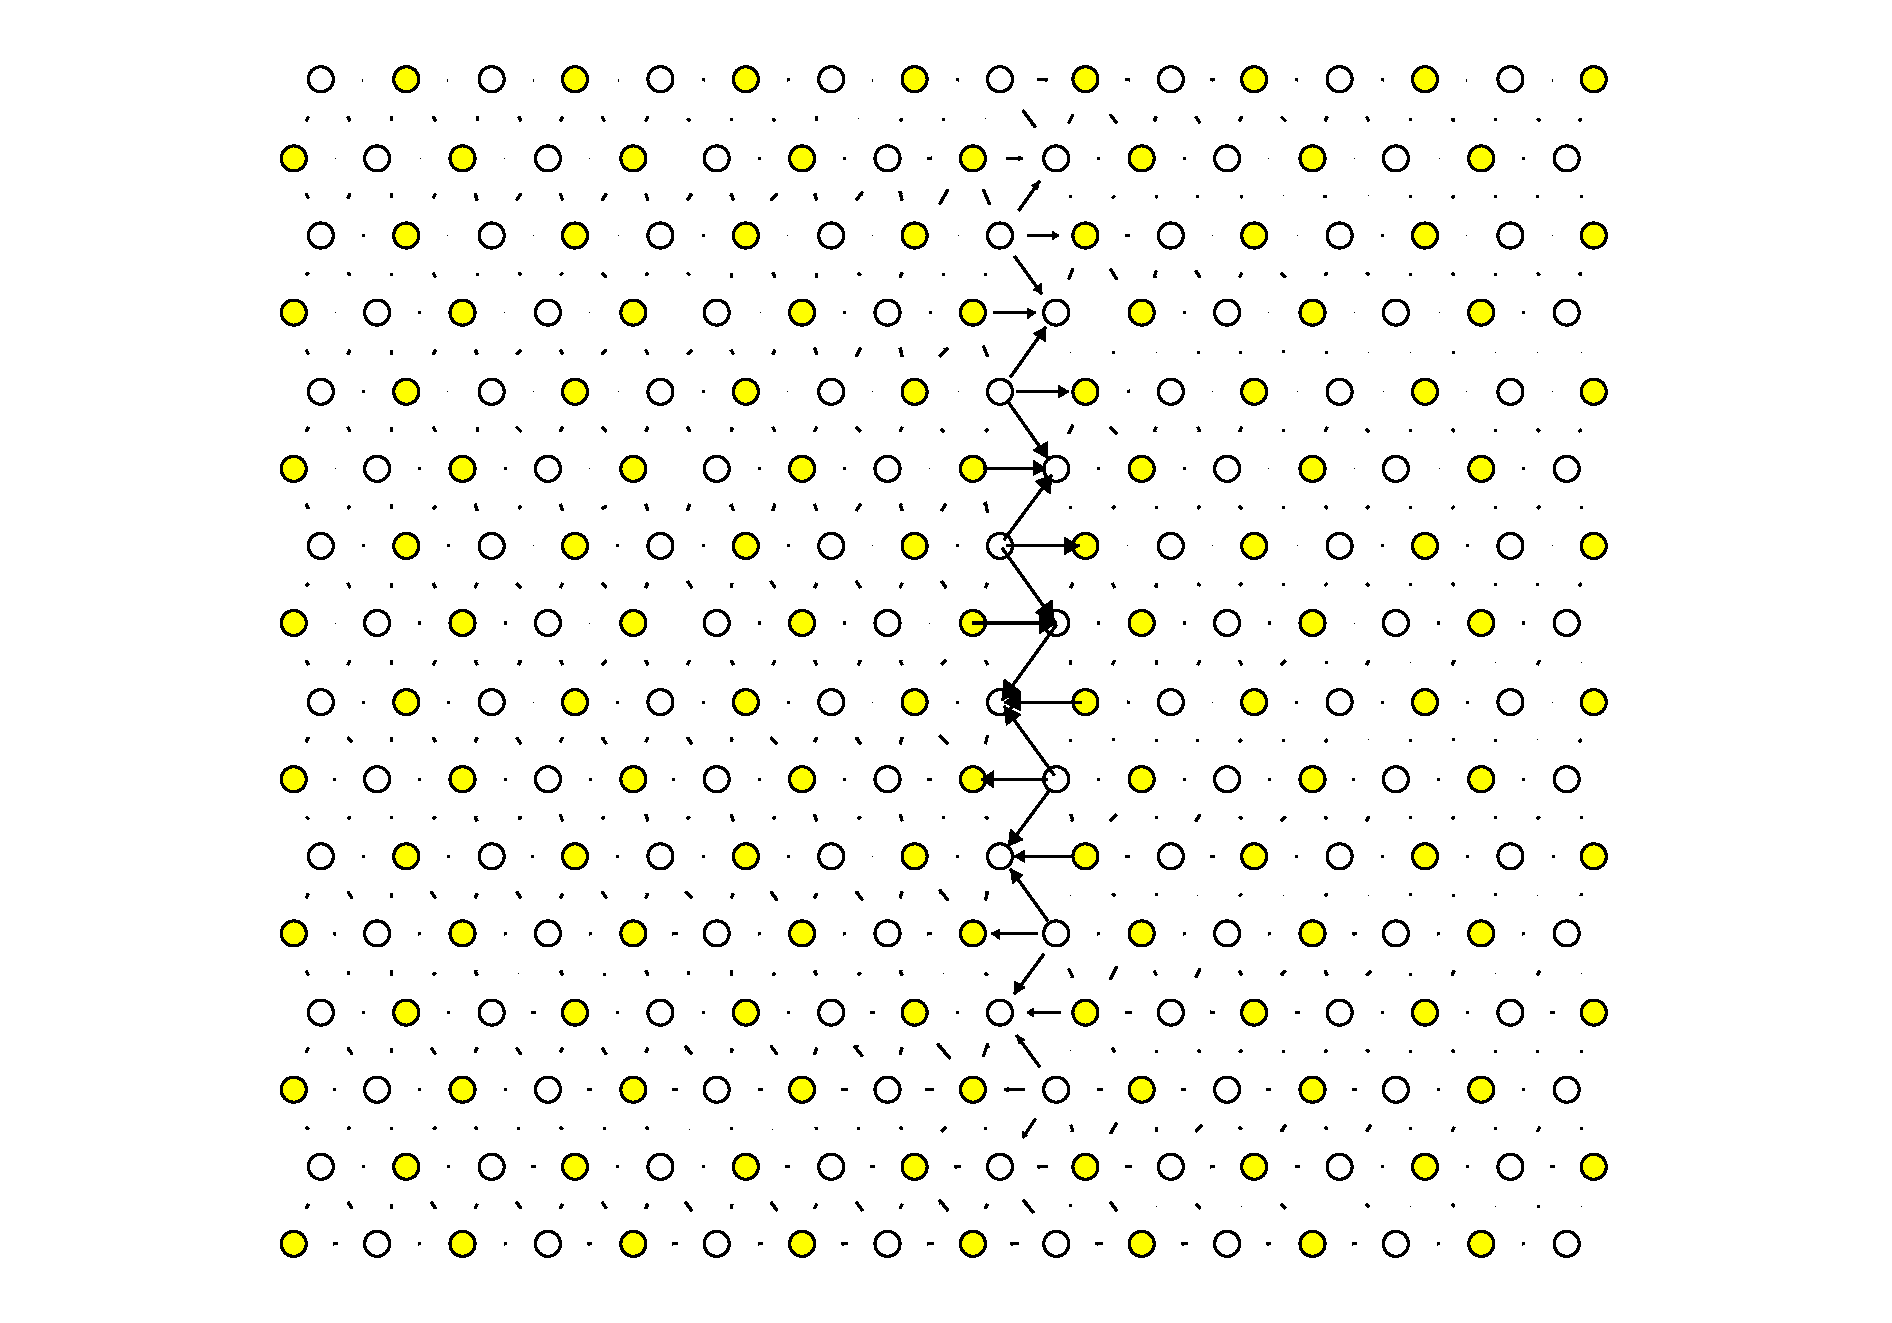
\includegraphics[width=.9\linewidth]{Images/ddplot_IP3_noo_best_model_alat.eps}
\end{center}
\begin{center}
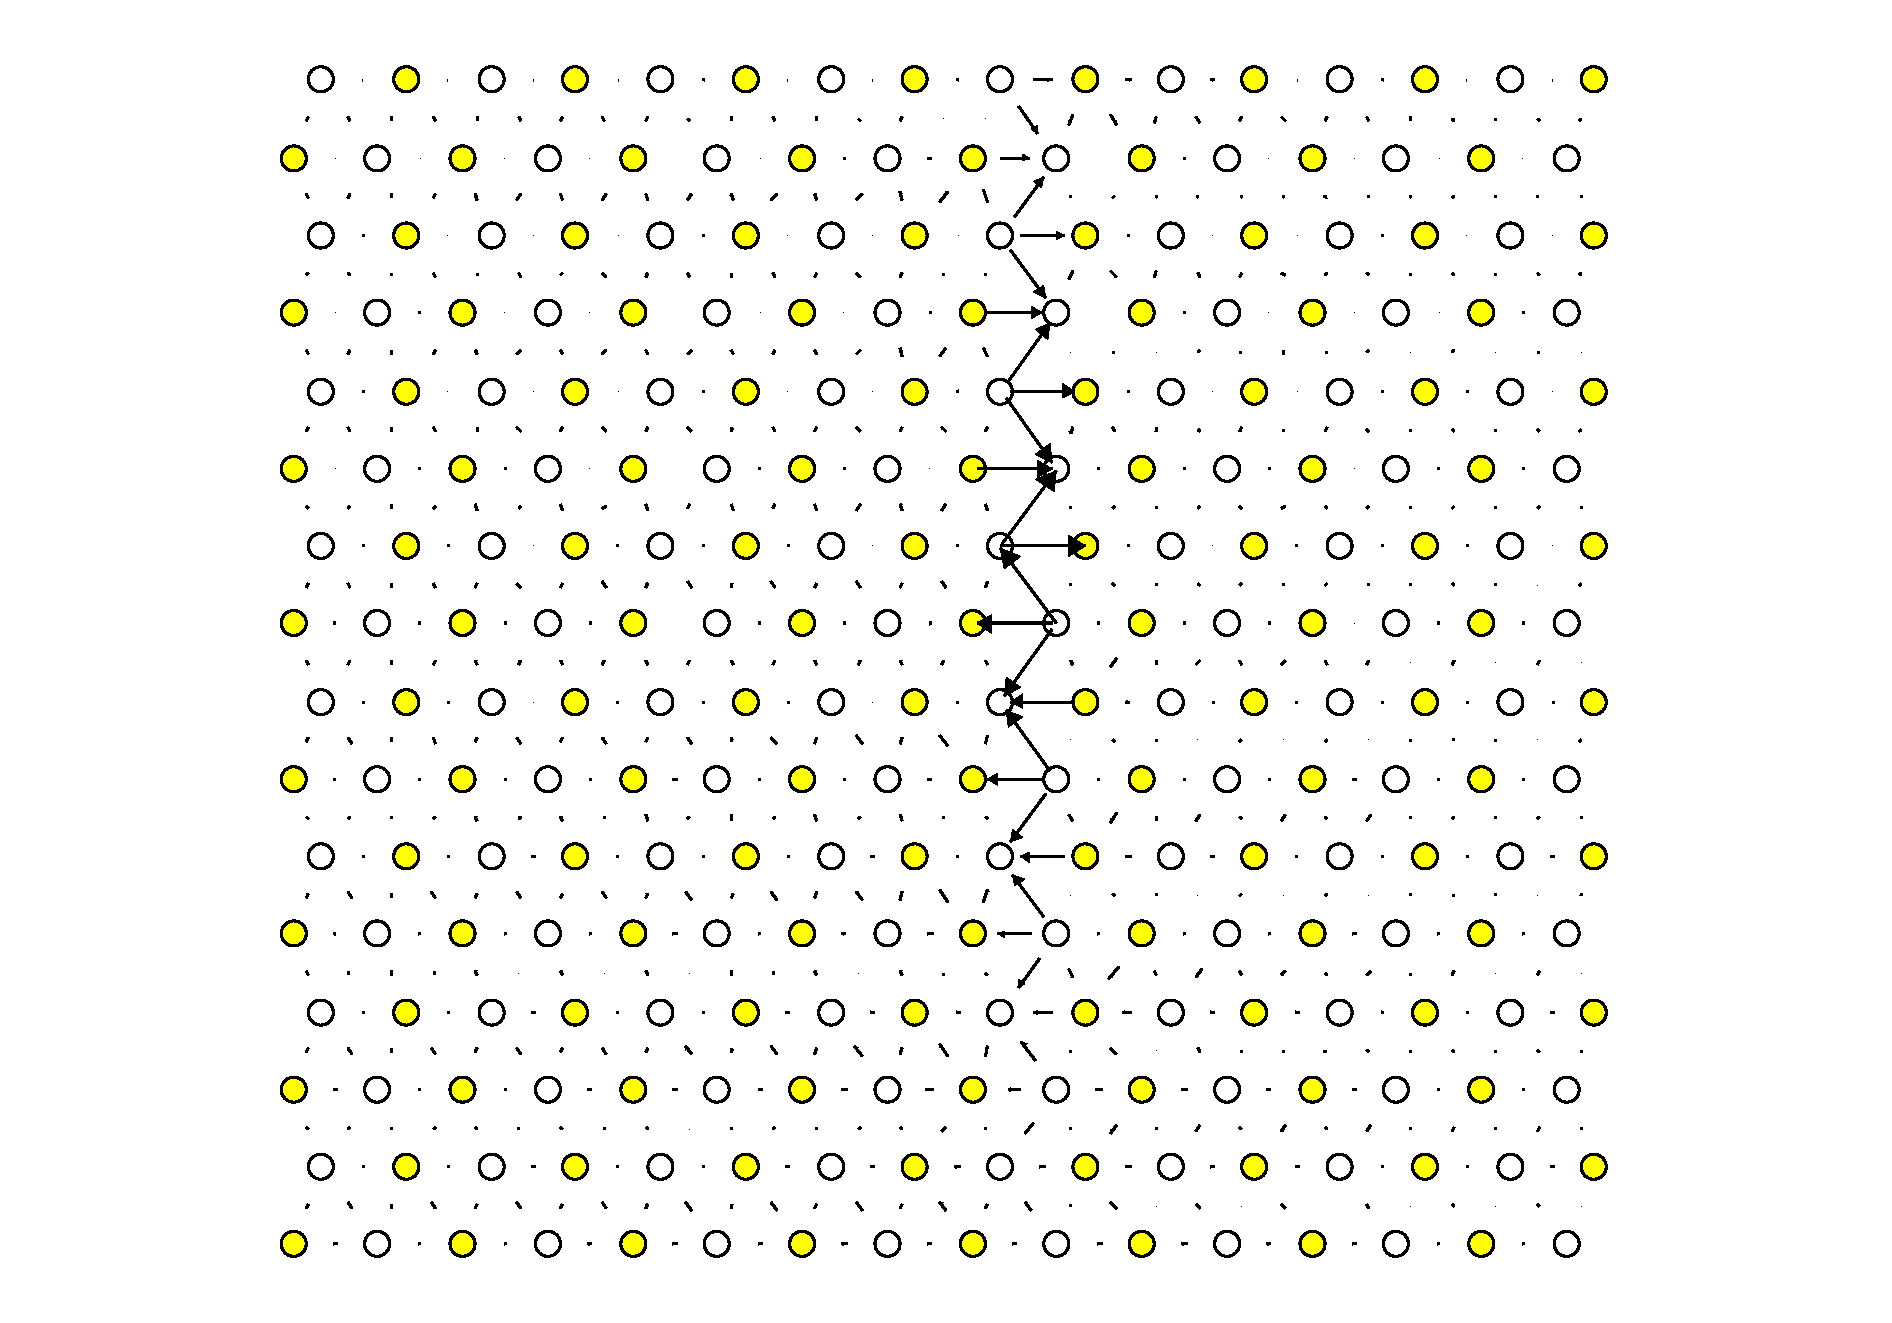
\includegraphics[width=.9\linewidth]{Images/ddplot_IP4_noo_best_model_alat.eps}
\end{center}
\begin{center}
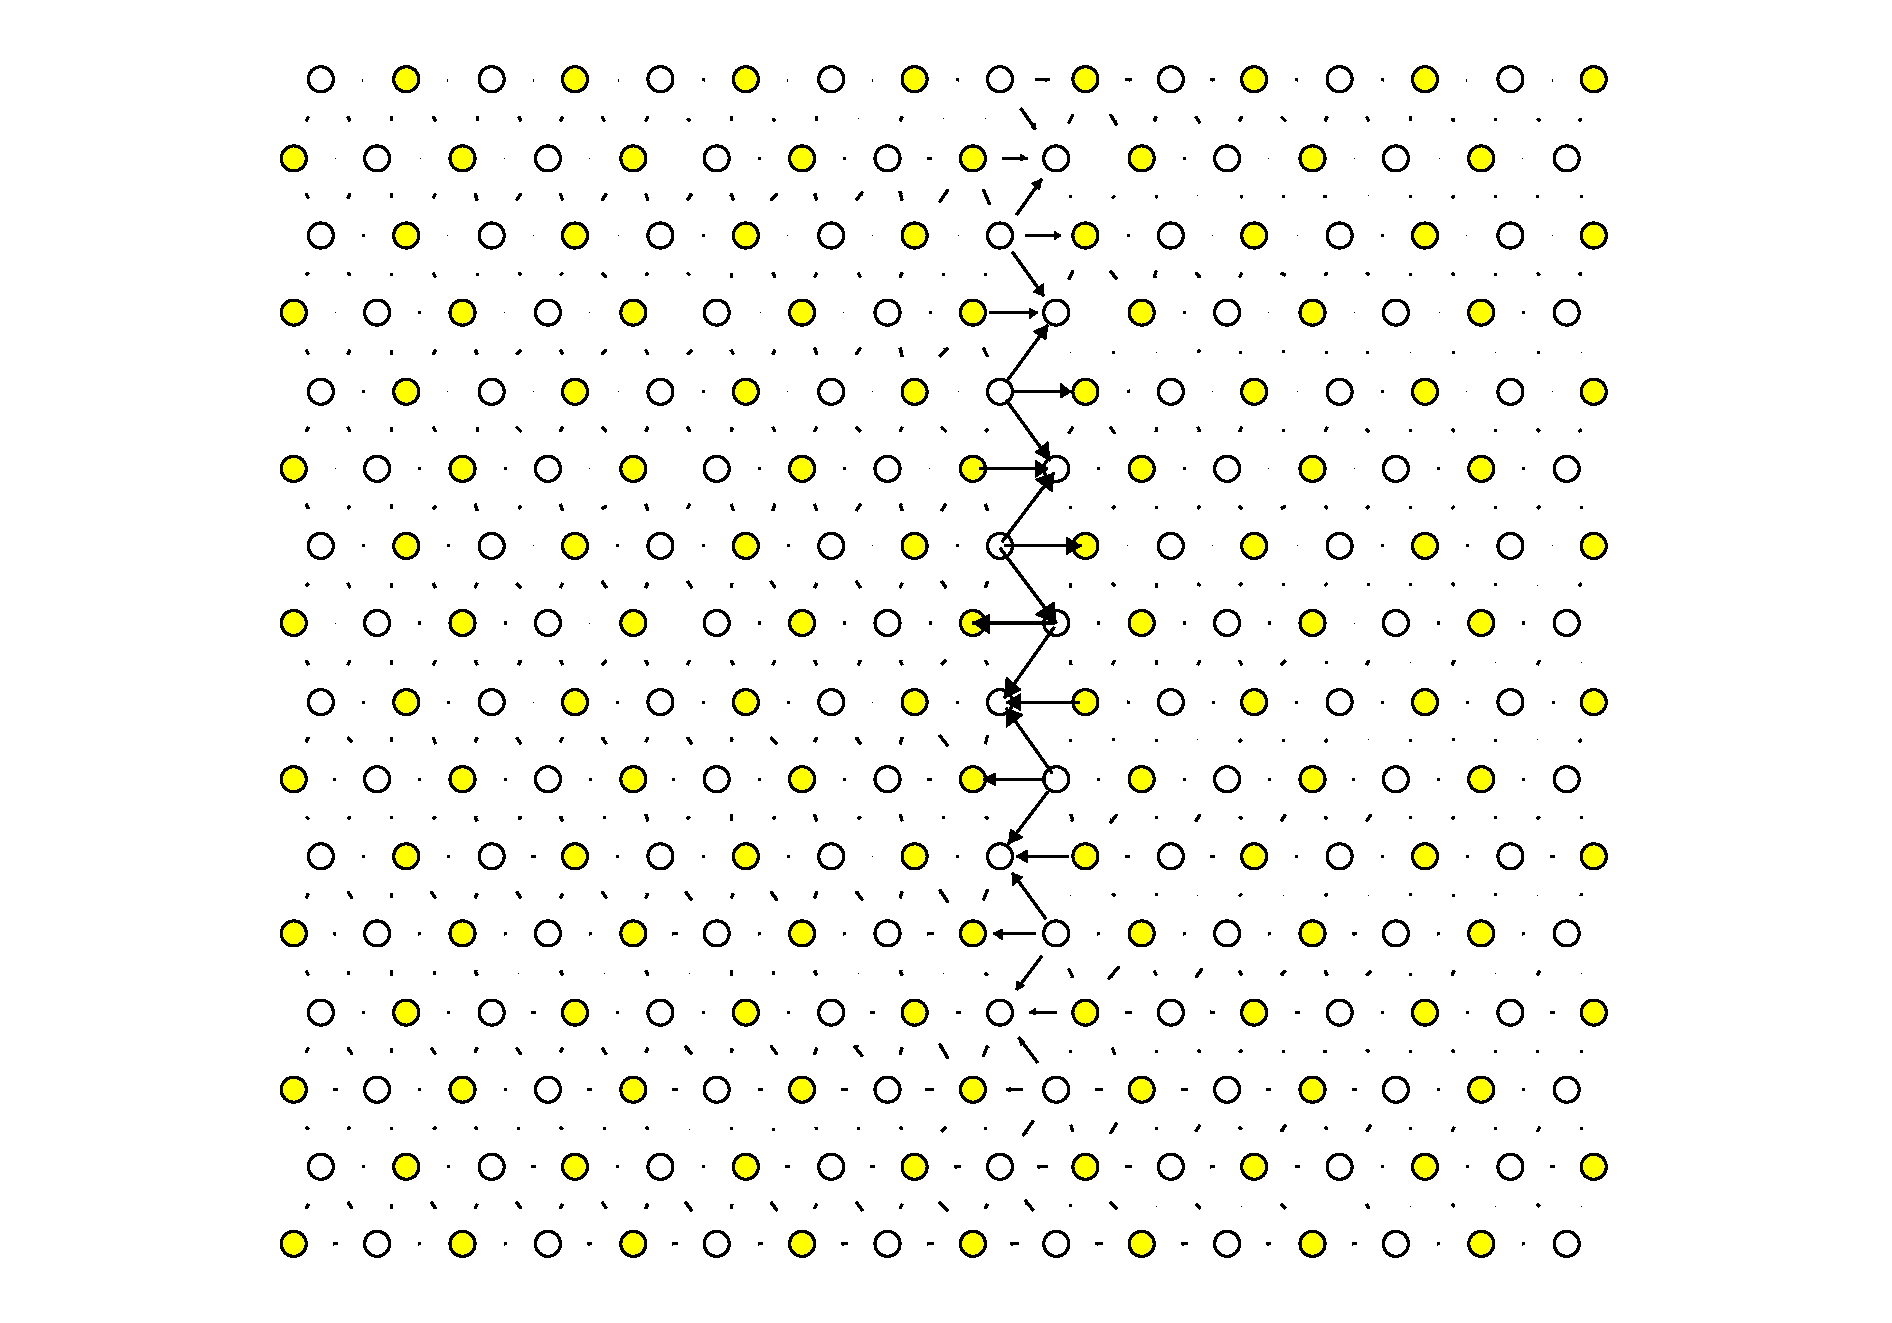
\includegraphics[width=.9\linewidth]{Images/ddplot_IP5_noo_best_model_alat.eps}
\end{center}

\begin{enumerate}
\item Data
\label{sec:org12ebd27}
\href{file:///home/tigany/Documents/ti/final\_model\_2019-11-12/results\_2019-11-09\_muc/IP1-oo\_19-11-09--04-46-00.log}{IP1}
\href{file:///home/tigany/Documents/ti/final\_model\_2019-11-12/results\_2019-11-09\_muc/IP2-oo\_19-11-09--04-46-00.log}{IP2}
\href{file:///home/tigany/Documents/ti/final\_model\_2019-11-12/results\_2019-11-09\_muc/IP3-oo\_19-11-09--04-46-00.log}{IP3}
\href{file:///home/tigany/Documents/ti/final\_model\_2019-11-12/results\_2019-11-09\_muc/IP4-oo\_19-11-09--04-46-00.log}{IP4}
\href{file:///home/tigany/Documents/ti/final\_model\_2019-11-12/results\_2019-11-09\_muc/IP5-oo\_19-11-09--04-46-00.log}{IP5}
\end{enumerate}

\subsubsection{Directory of the results}
\label{sec:org52f87b4}
\url{file:///home/tigany/Documents/ti/2019-09-11\_final\_model/tbe/dislocations/2019-11-08\_no\_omega\_ordering\_ec\_latpar/}
\url{file:///home/tigany/Documents/ti/final\_model\_2019-11}

\subsubsection{BOP}
\label{sec:org46d7a82}

\begin{enumerate}
\item 4 recursion levels
\label{sec:orgf84cee0}

kbT = 0.1

>> Lattice parameters:

> hcp
\begin{center}
\begin{tabular}{ll}
a & 2.901660  \AA{}\\
c & 4.747485  \AA{}\\
etot & -18.342162  eV\\
\end{tabular}
\end{center}

> omega
\begin{center}
\begin{tabular}{ll}
a & 7.917318  \AA{}\\
c & 2.749892 \AA{}\\
etot & -17.458700 eV\\
\end{tabular}
\end{center}

Omega is still not as stable as hcp as expected from model. 


>> Elastic Constants

\begin{center}
\begin{tabular}{lrr}
Quantity & calc. (10\(^{\text{11}}\) Pa) & exp. (10\(^{\text{11}}\) GPa)\\
\hline
C11 & 1.781 & 1.761\\
C12 & 0.738 & 0.868\\
C13 & 0.611 & 0.682\\
C33 & 1.969 & 1.905\\
C44 & 0.285 & 0.508\\
C66 & 0.522 & 0.450\\
K & 1.050 & 1.101\\
R & 0.669 & 0.618\\
H & 0.558 & 0.489\\
\end{tabular}
\end{center}
\end{enumerate}
\end{document}